\documentclass{article}
\usepackage[utf8]{inputenc}
\usepackage{graphicx}
\usepackage{subfig}
\usepackage{parskip}

\setlength{\parskip}{1em}

\title{Fichero Aclaratorio}
\author{Pablo Rodriguez Guillen \\ \\ Profesor: Enrique García Salcines}
\date{Abril 2019}

\begin{document}

\maketitle

\renewcommand\thesection{}

\section{Ejercicio 1}
En primer lugar comprueba que los argumentos introducidos por el usuario son correctos. Si no lo son se imprime un mensaje de error en el que se especifica el formato del comando para ejecutar el script correctamente.\par
Si la ejecución por parte del usuario es correcta, se cuentan los ficheros con extensión ".c" y ".h" usando el comando find con la opción -name y se imprime la información obtenida por pantalla.\par
Posteriormente, haciendo uso de un bucle for se itera por cada uno de los ficheros del directorio especificado. En cada iteración se obtienen el número de líneas y de caracteres y se imprime por pantalla dicha información. Esta impresión se ordena por el número de caracteres de mayor a menor de cada fichero, haciendo uso del comando sort.\par
Una ejecución del script se mostraría así:

\begin{figure}[ht]
    \centering
    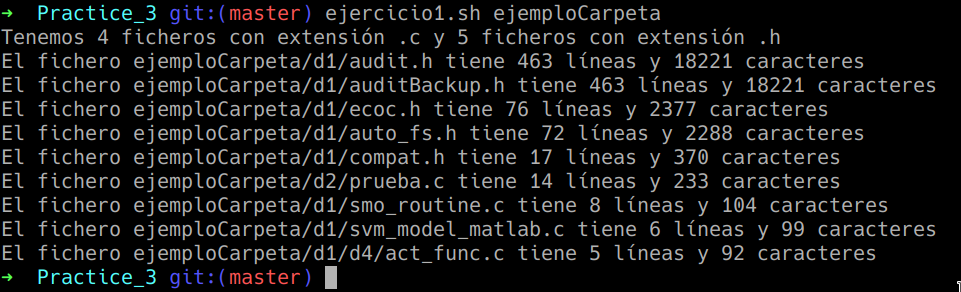
\includegraphics[width=1\textwidth]{ejercicio1.png}
    \caption{Ejecución ejercicio1.sh}
\end{figure}

\section{Ejercicio 2}
Al igual que en el ejercicio 1 y en el resto de los de la práctica. Se comprueba que los argumentos son correctos y si no lo son se imprime un mensaje de error. También se asigna un valor por defecto al argumento opcional.\par
En el bucle for, se recorre cada uno de los ficheros del directorio especificado. En cada iteración se crean dos variables locales: LongitudUsuario y Ejecutable. El resto de parámetros a mostrar tienen una obtención directa mediante opciones del comando stat.\par
Al igual que en el ejercicio anterior, se hace uso de una tubería para ordenar la salida por pantalla. Cabe mencionar que se hace uso de la opción -t para definir un carácter separador (";" en este caso). La salida se ordena por el tamaño en bytes del fichero de menor a mayor.\par
La ejecución del script se mostraría así:

\begin{figure}[ht]
    \centering
    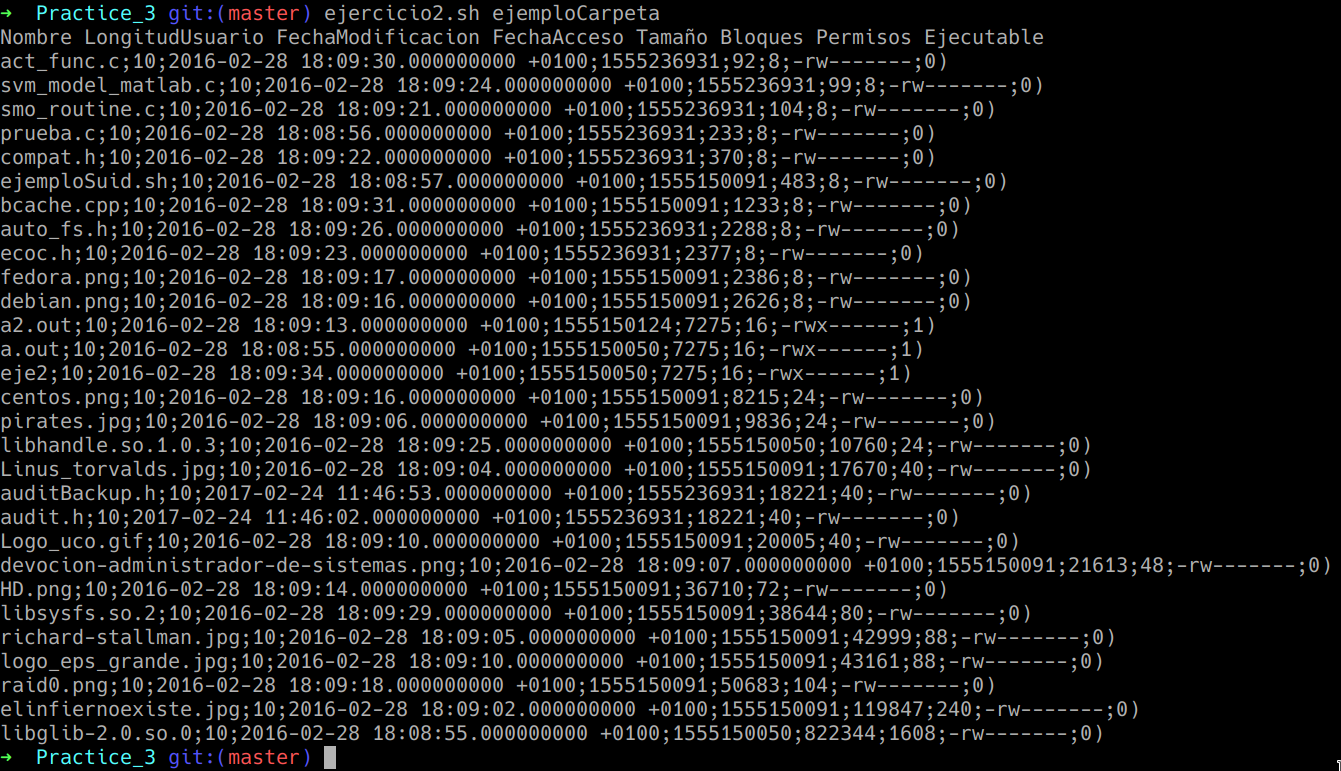
\includegraphics[width=1\textwidth]{ejercicio2.png}
    \caption{Ejecución ejercicio2.sh}
\end{figure}

\section{Ejercicio 3}
En primer lugar se realizan la comprobación ya mencionada de argumentos y la posterior asignación de valores por defecto a los argumentos opcionales. Estos, son los 2 números de bytes por los que se van a dividir los ficheros. Dado que uno debe ser mayor que el otro, se ha añadido un if que intercambie los valores si el usuario introduce el mayor antes que el menor.\par
En segundo lugar, se procede a la creación de las carpetas "pequenos", "medianos" y "grandes" si estas carpetas no existían previamente. Si este fuera el caso, el script borra las carpetas y las vuelve a crear. Ambas acciones se imprimen por pantalla.\par
Por último, se hacen 3 bucles for que se diferencian por el uso de la opción -size del comando find en el que se copian a la carpeta que correspondan los ficheros que cumplan las condiciones del find.\par
Así se verían 2 ejecuciones del script, una con los valores por defecto y otra estableciendo el umbral inferior a 11000 bytes:

\begin{figure}[ht]
    \centering
    \subfloat[Valores por defecto]{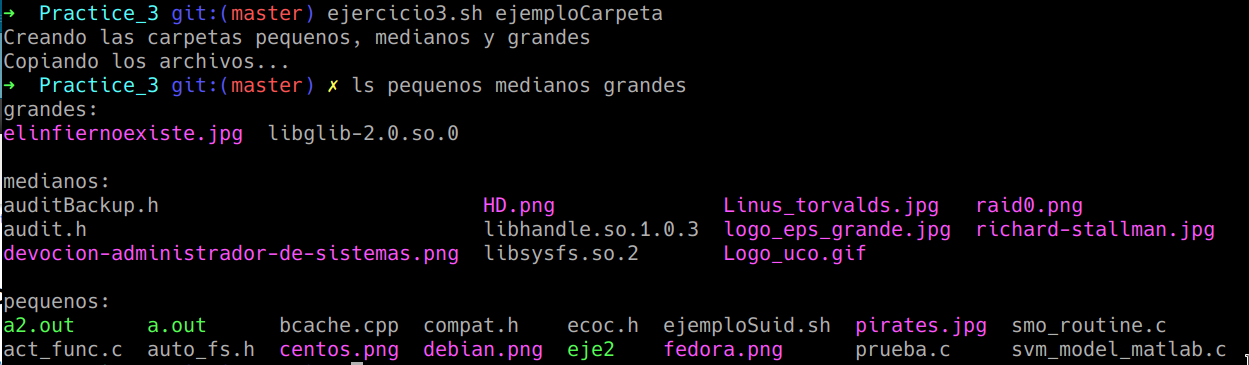
\includegraphics[width=1\textwidth]{ejercicio3-1.png}}\qquad
    \subfloat[Umbral inferior 11000]{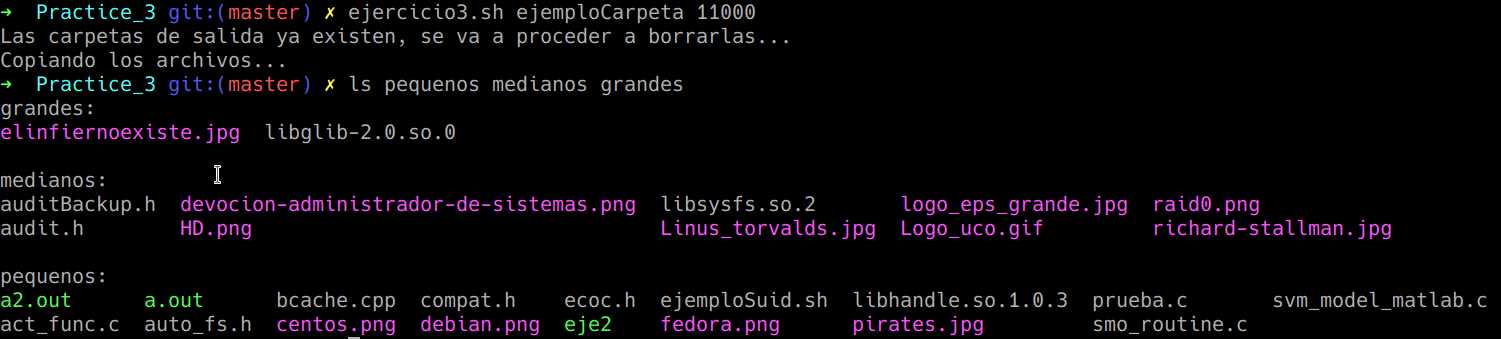
\includegraphics[width=1\textwidth]{ejercicio3-2.png}}
    \caption{Ejecución ejercicio3.sh}
\end{figure}

\section{Ejercicio 4}
Este script no cuenta con argumentos y utiliza como directorio sobre el que actuar, el directorio actual del usuario.\par
En primer lugar, usa el comando find con la opción -maxdepth=1 para contar el número de ficheros en el directorio actual. La información se imprime por pantalla.
En segundo lugar, haciendo uso del comando awk, imprime los usuarios logueados en el sistema sin repetirlos (comando uniq).\par
Posteriormente, pide al usuario que introduzca un carácter. Si este no lo introduce en 5 segundos, se asigna a la variable char el carácter "a". El script, usando un bucle for y el comando find recorre todos los ficheros del directorio, buscando en su nombre el carácter introducido. Usando grep, wc y tuberías se obtiene el número de apariciones de un carácter. Se introducen los datos en un fichero temporal que se borra al finalizar el script porque no he conseguido guardar el valor en una variable.\par
A continuación se muestran un par de ejecuciones del script:

\begin{figure}[ht]
    \centering
    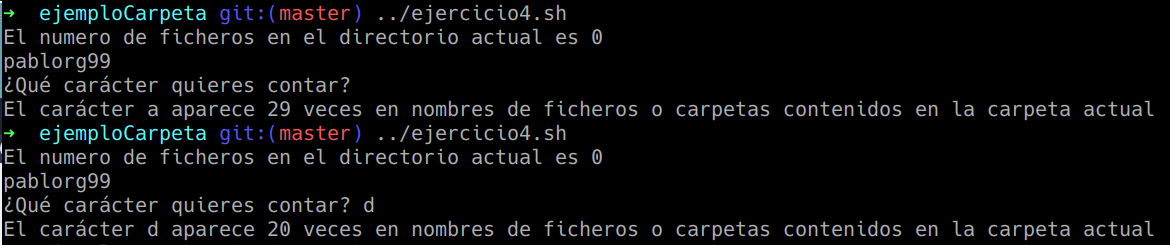
\includegraphics[width=1\textwidth]{ejercicio4.png}
    \caption{Ejecuciones ejercicio4.sh}
\end{figure}

\section{Ejercicio 5}
Este script comprueba si existe la carpeta "Copia" en el directorio home del usuario. Si no existe la carpeta se crea.\par
En segundo lugar, recorre los ficheros de la carpeta "Copia" comparando la fecha del último acceso con la fecha actual, si la diferencia es superior a 200 segundos, se borra la copia en cuestión. \par
Por último, se crea una copia de seguridad de los ficheros que se pasan como argumento en el directorio citado usando el comando tar. \par
A continuación se muestran 2 ejecuciones del script: 

\begin{figure}[ht]
    \centering
    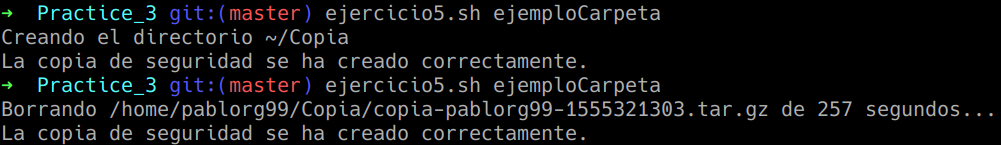
\includegraphics[width=1\textwidth]{ejercicio5.png}
    \caption{Ejecuciones ejercicio5.sh}
\end{figure}

\section{Ejercicio 6}
Tras comprobar que los argumentos son correctos, el script escribe en un fichero html el título y la cabecera del mismo. Cuando va a escribir el cuerpo, hace una llamada a la función listFile con el argumento pasado por el usuario. \par
En la función, se abre una enumeración html con la etiqueta \textless ul\textgreater \space y se recorren los ficheros del directorio pasado como argumento. Si el fichero de una iteración es un directorio, se escribe en negrita y se hace una llamada recursiva a listFile, si no, se escribe normal. Ambas escrituras se hacen con la etiqueta  \textless li\textgreater .
A continuación se muestran imágenes del fichero html creado tanto en el editor como en el navegador. El argumento pasado al script es "ejemploCarpeta":

\begin{figure}[ht]
	\centering
	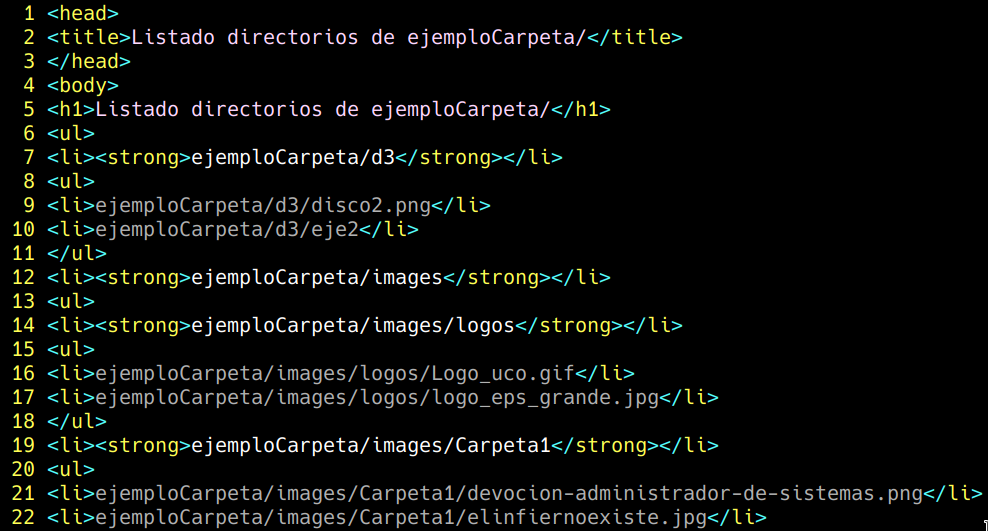
\includegraphics[width=1\textwidth]{ejercicio6-1.png}
	\caption{Fichero html en editor}
\end{figure}

\begin{figure}[ht]
	\centering
	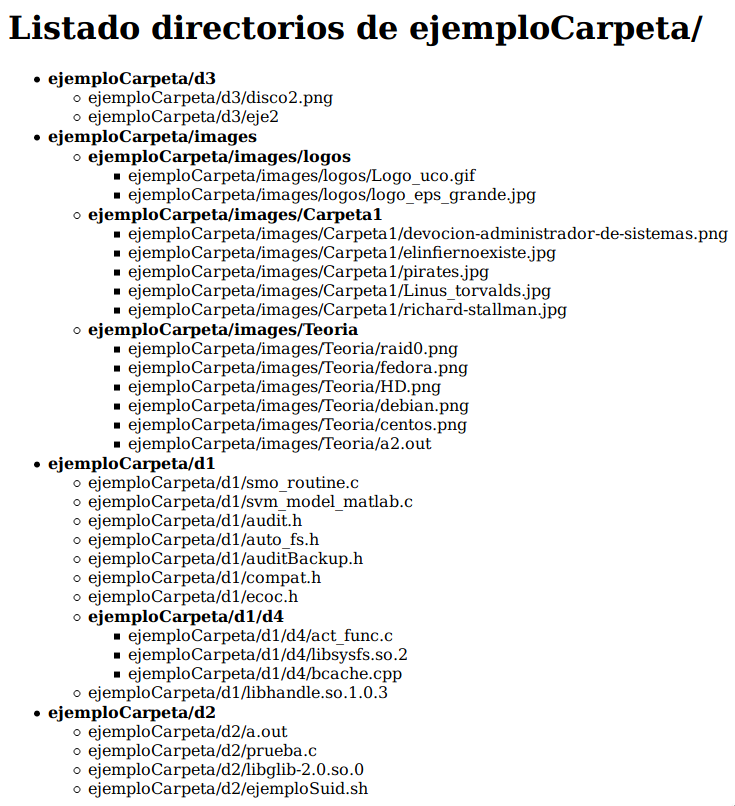
\includegraphics[width=1\textwidth]{ejercicio6-2.png}
	\caption{Fichero html en navegador}
\end{figure}


\end{document}
